\section*{Remerciements}

Ce rapport de stage a été réalisé dans le cadre du projet ECOVERGER, action pilotée par le ministère de l’Agriculture et de l’alimentation et le ministère de la Transition écologique et solidaire, avec l’appui financier de l’Agence française pour la biodiversité dans le cadre de l'APR «Résistance et pesticides» grâce aux crédits issus de la redevance pour pollutions diffuses attribués au financement du plan Ecophyto et dans le cadre du programme de recherche agronomique du Cirad à la Réunion, DPP COSAQ, (activités 2015-2018) financé par la communauté européenne (fond structurel FEDER) et le Conseil Régional de La Réunion.





\begin{figure}[!h]
 \centering
 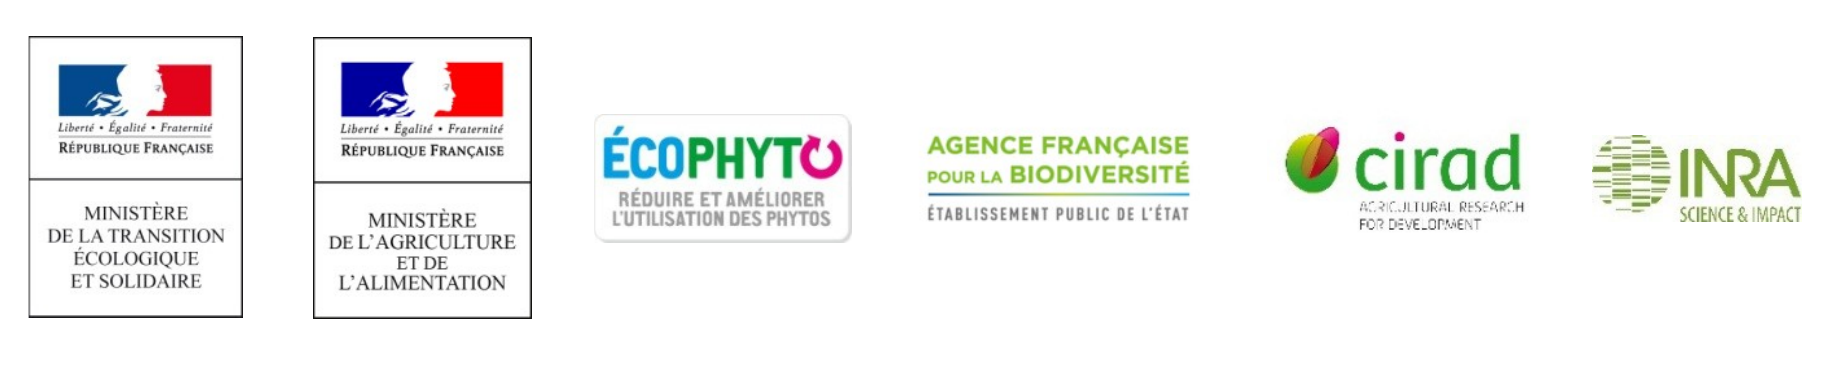
\includegraphics[scale = 0.3]{photos/ecoverger.png}
\end{figure}



\begin{figure}[!h]
 \centering
 
\includegraphics[scale = 0.3]{photos/cosaq.png}
\end{figure}
